\documentclass{ikpKoeln}
\usepackage{graphicx}
\usepackage{physics}
\usepackage{xcolor}
\usepackage{tikz}
\usetikzlibrary{math}

\scTitle{NeuLAND calibration revisit: Millepede algorithm and error analysis of map2cal calibration}
\scAuthor{*}{Yanzhao}{Wang}{1}
\scAffiliation{1}{University of Cologne, Institute for Nuclear Physics, Germany}

\scTitleShort{NeuLAND Meeting 05.04.2024}

\date{\scriptsize NeuLAND weekly meeting \\ 05.04.2024}

\graphicspath{{../figures/}}

\addbibresource{reference.bib}

\begin{document}

\begin{frame}{Overview}
	\begin{itemize}
		\Large
		\setlength\itemsep{2em}
		\item Statistical error analysis of TDC calibration
		\item Millepede algorithm principle
		\item Millepede algorithm application to NeuLAND
		\item Preliminary results
	\end{itemize}
\end{frame}

\begin{frame}[t]{NeuLAND TDC calibration}
	\vspace*{-0.5em}
	\begin{columns}[t]
		\begin{column}{0.45\textwidth}
			\vspace*{-2em}
			\begin{block}{TDC calibration relation:}
				\small
				$f(x)$: Channel number $\Longrightarrow$ Time value (ns)
			\end{block}
			\begin{figure}
				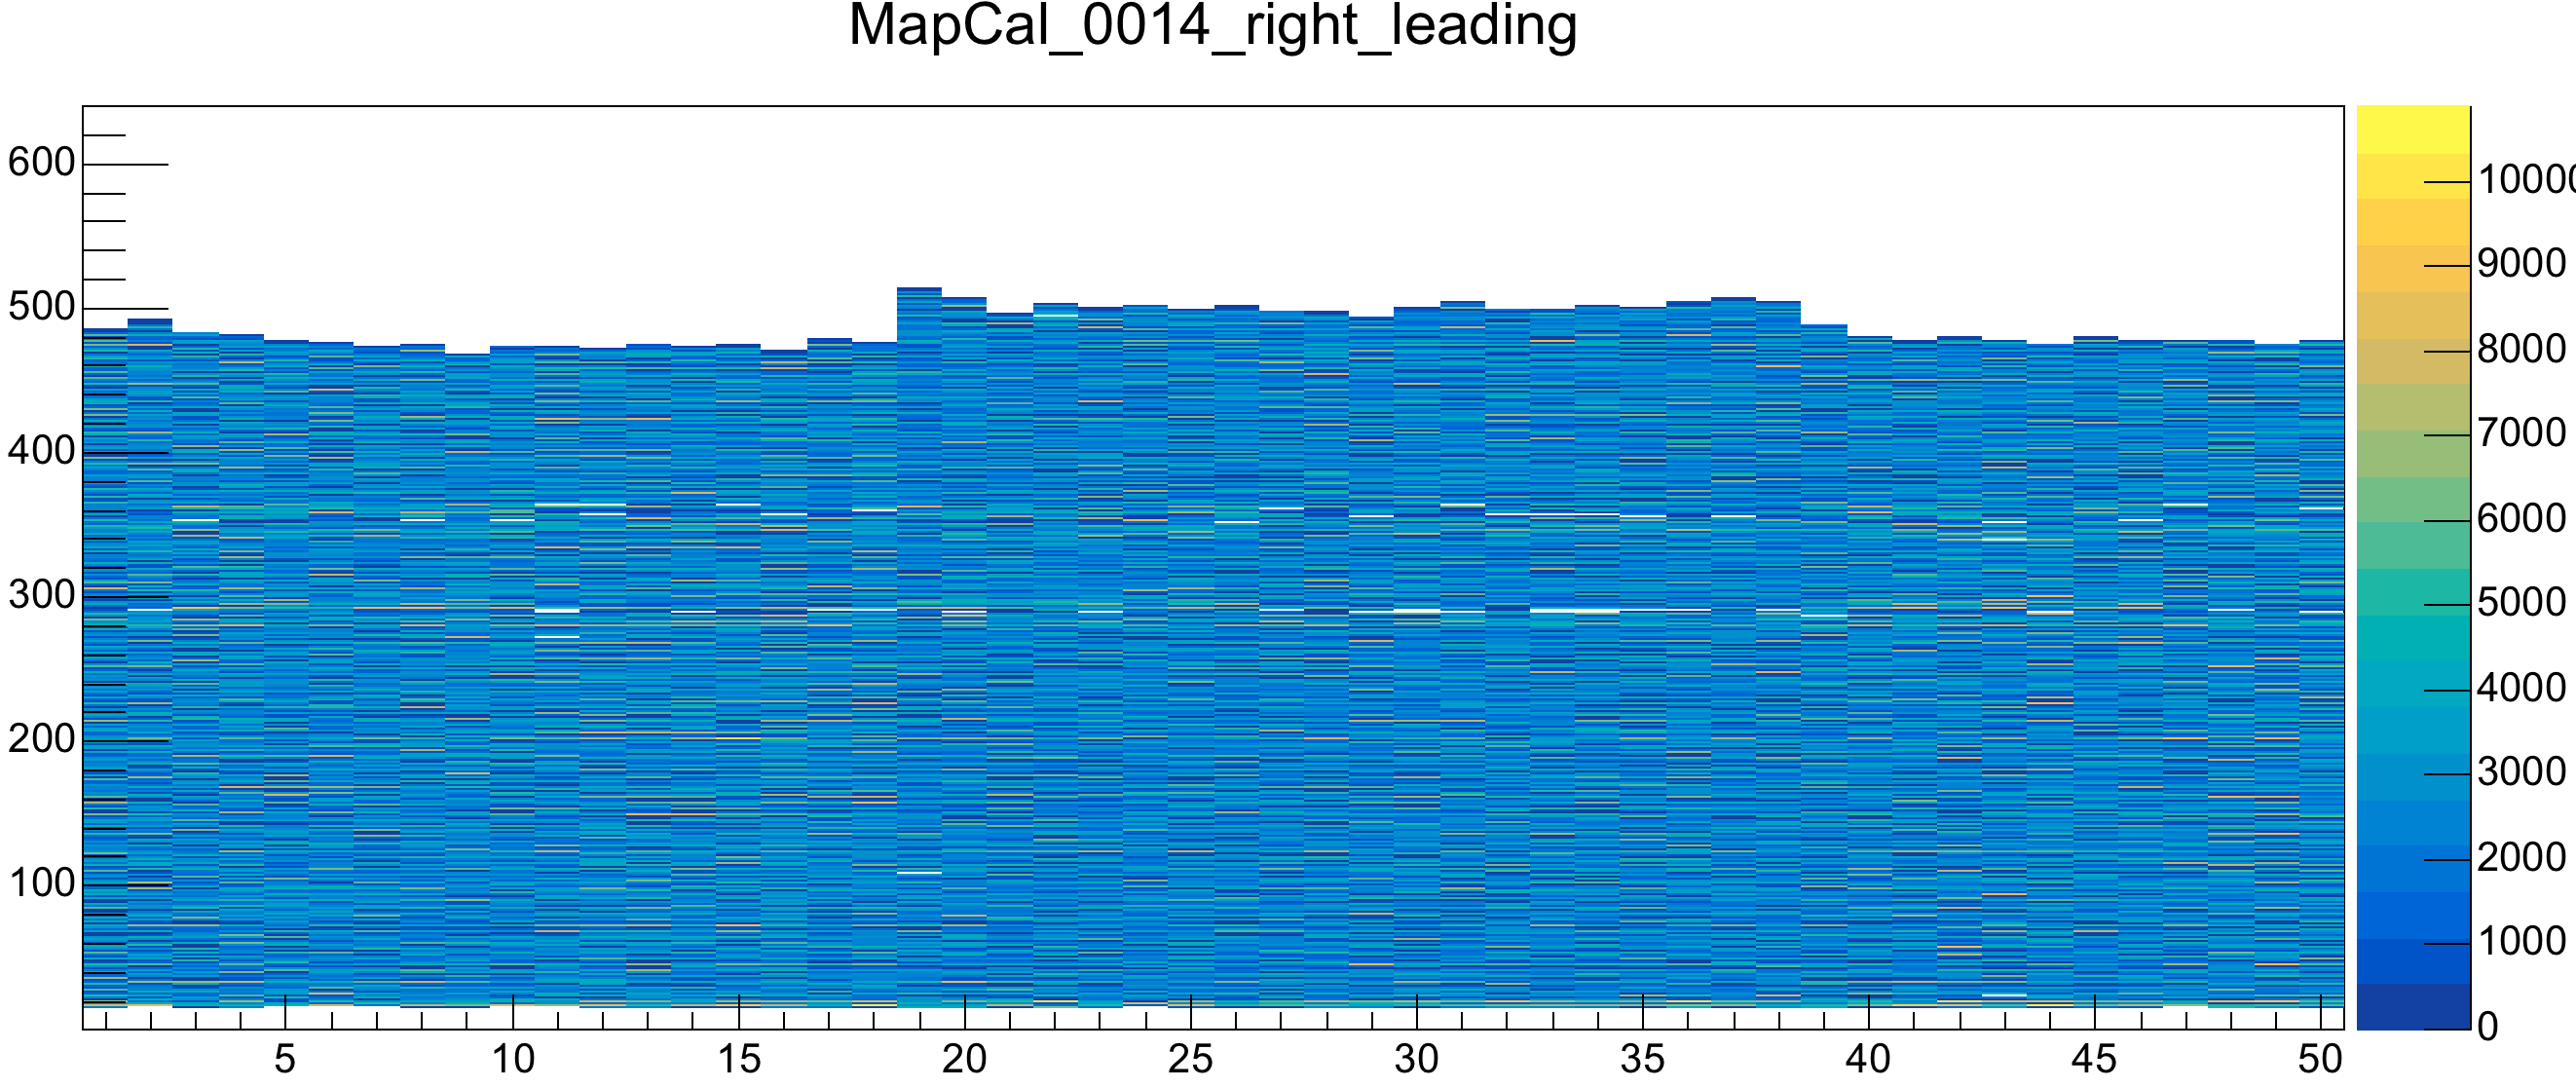
\includegraphics[width = \textwidth]{ neulandMeeting/mapcal_plane_distri.png}
				\vspace*{1em}
				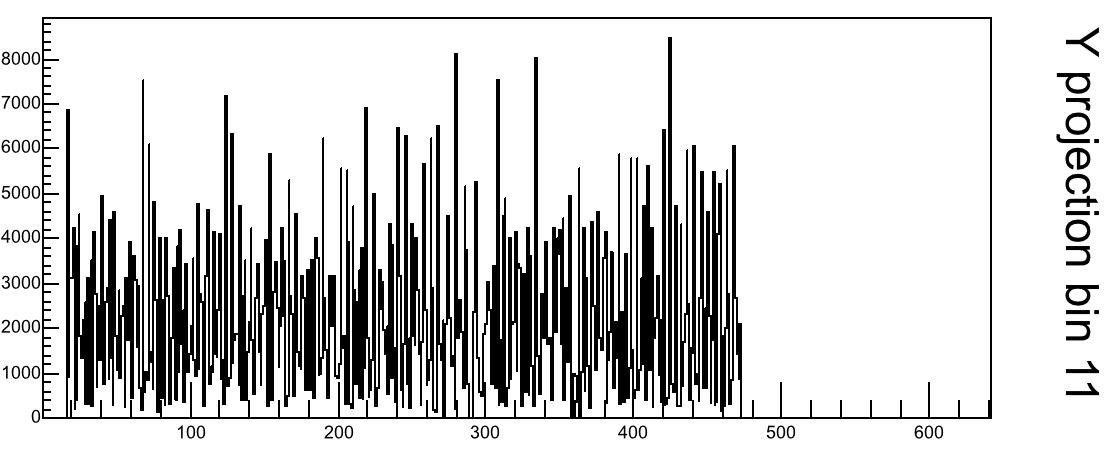
\includegraphics[width = \textwidth]{ neulandMeeting/mapcal_bar_dsistri.png}
			\end{figure}
		\end{column}
		\begin{column}{0.45\textwidth}
			\textit{\small Two time components:}
			\begin{itemize}
				\scriptsize
				\item coarse time ($\pm$ 5 ns)
				\item fine time ($\pm$ 10 ps)
			\end{itemize}
			\textit{\small Fine time Calibration procedures:}
			\begin{enumerate}
				\scriptsize
				\item Collection of of all TDC values
				\item Calculation of cumulative distribution of TDC values
				\item Scaling of CFD to $0\sim5$ ns
			\end{enumerate}
			\vspace*{-1em}
			\flushleft \scriptsize{CDF:}
			\begin{figure}
				\vspace*{-1em}
				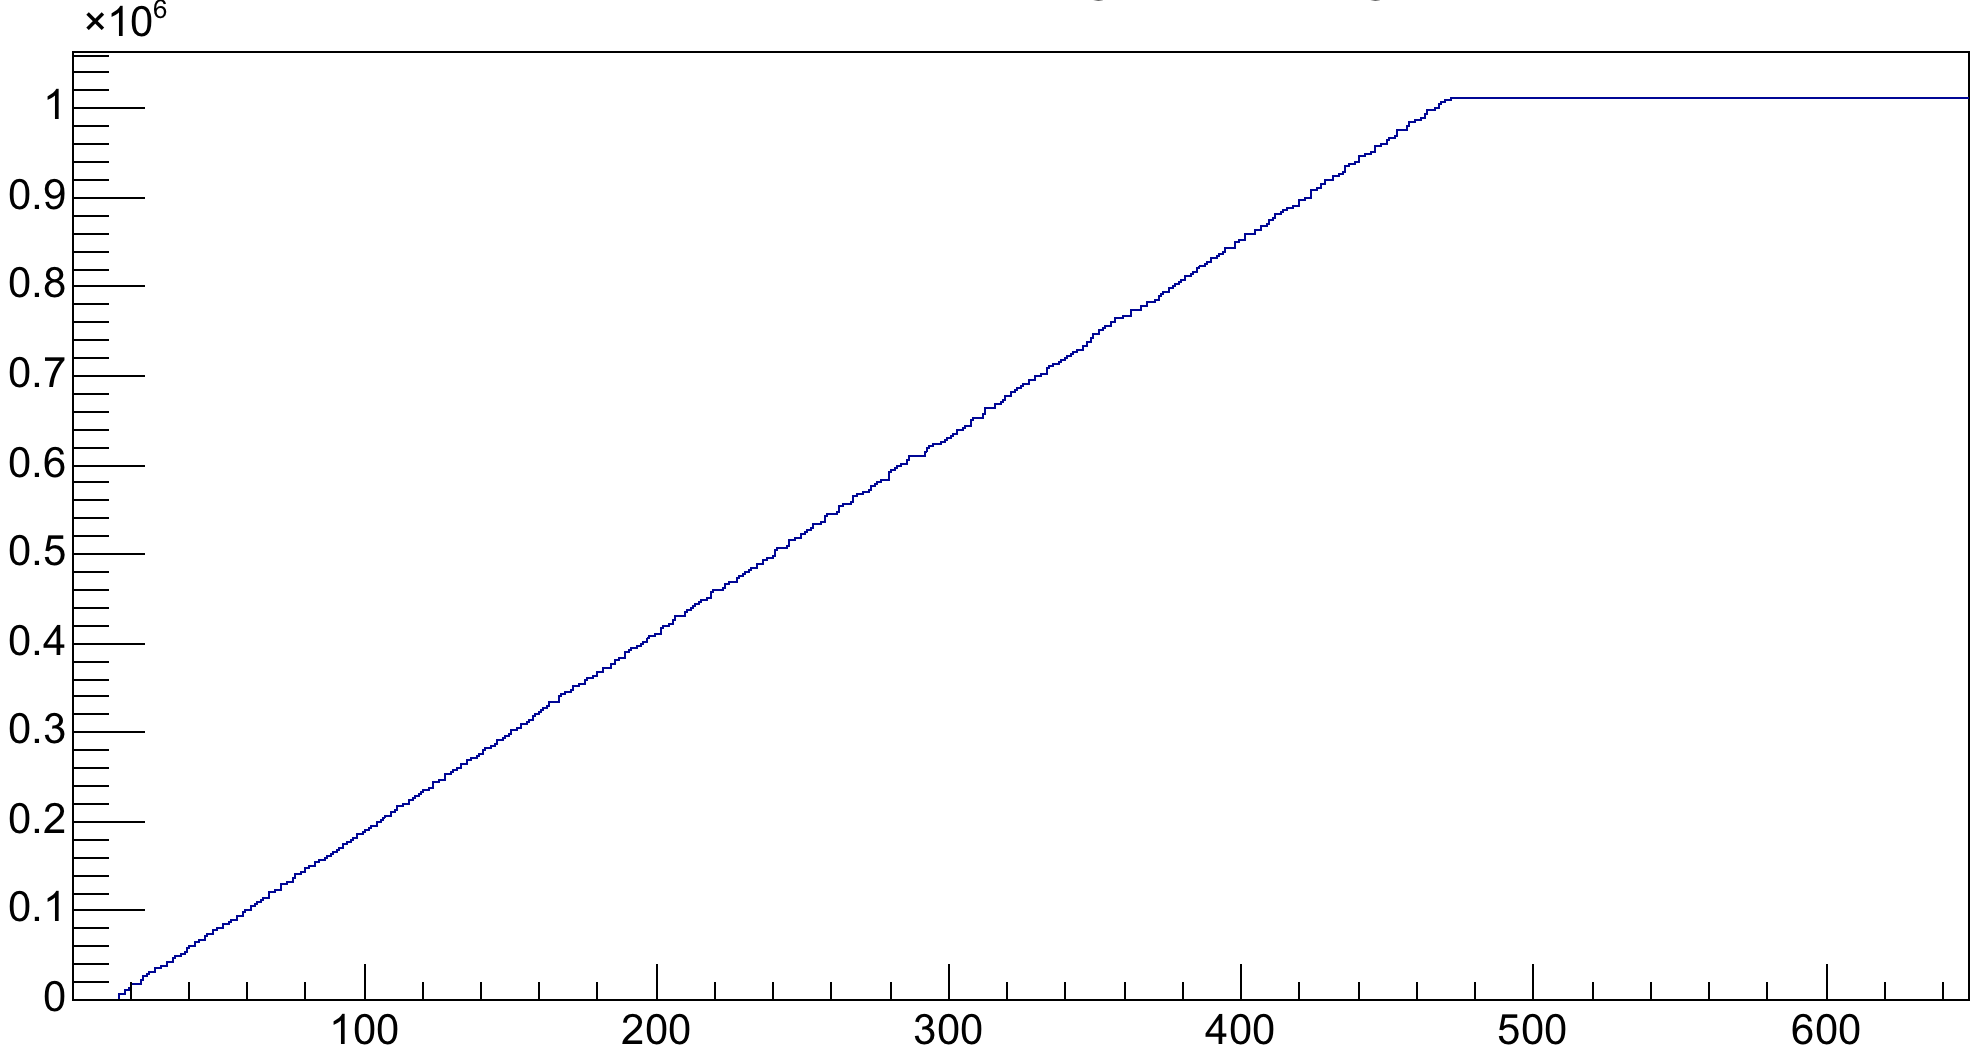
\includegraphics[width = \textwidth]{ neulandMeeting/mapcal_cumulative.png}
			\end{figure}
		\end{column}
	\end{columns}
\end{frame}

\begin{frame}[t]{Statistical error analysis of TDC calibration}
	\flushleft \textbf{Convolution of two distributions:}
	\begin{itemize}
		\item Uniform distribution: fine time $\sim \mathcal{U}(f(n), f(n + 1))$
		\item Multinomial distribution: $f(n), f(n+1) \sim \mathcal{M}_k(3,p_a, p_b), \ p_a = \text{CDF}(n), p_b = \text{PDF}(n)$
	\end{itemize}

	\flushleft \textbf{Mathematical derivation:}
	\flushleft {\small Mean:}
	\scriptsize{
		$$ E(X) = \sum_{n_a, n_b} \mathcal{M}(n_a,n_b;3,p_a, p_b) \cdot \int_{n_a}^{n_b} xf(x) \,dx = \bar{n_a} + \bar{n_b} / 2 $$
	}
	\flushleft {\small Variance:}
	{
		\scriptsize
		\begin{align*}
			Var(X) & = E(X^2) - E^2(X)                                                                                                                                                      \\
			E(X^2) & = \sum_{n_a, n_b} \mathcal{M}(n_a,n_b;3,p_a, p_b) \cdot \int_{n_a}^{n_b} x^2f(x) \,dx = \sum_{n_a, n_b} \mathcal{M}(n_a,n_b;3,p_a, p_b)(n_a^2n_b + n_an_b^2 + n_b^2/3) \\
			       & = Var(N_a) + E^2(N_a) + Cov(N_a, N_b) + E(N_a)E(N_b) + \left(Var(N_a) + E^2(N_b)\right)/3                                                                              \\
			Var(X) & = N^2 p_b^2 / 12 + N \left( -(p_a - \frac{1-p_b}{2})^2 + 1/4 - p_b / 6 - p_b^2 /12 \right)
		\end{align*}
	}%

\end{frame}

\begin{frame}[t]{Validation of the error analysis}
	\begin{columns}[t]
		\begin{column}{0.5\textwidth}
			\begin{alertblock}{\small Exact solution (no approximation):}
				\centering
				\small$\delta = \sqrt{\frac{N^2p_b^2}{12} + N \left( -(p_a - \frac{1-p_b}{2})^2 + \frac{1}{4} - \frac{p_b}{6} - \frac{p_b^2}{12} \right)}$
			\end{alertblock}
			\begin{exampleblock}{\small Approximate solution:}
				\centering
				\small$\delta = \frac{Np_b}{\sqrt{12}} + \frac{\sqrt{3}}{p_b}(-(p_a - \frac{1}{2})^2 + \frac{1}{4})$ \,\,\, ($p_b \neq 0$)
			\end{exampleblock}
			\begin{block}{\small Base solution:}
				\centering
				\small$\delta = \frac{Np_b}{\sqrt{12}}$
			\end{block}
		\end{column}
		\begin{column}{0.45\textwidth}
			\vspace*{-1.5em}

			\flushleft \textit{Comparison to Monte-Carlo data:}
			\begin{figure}
				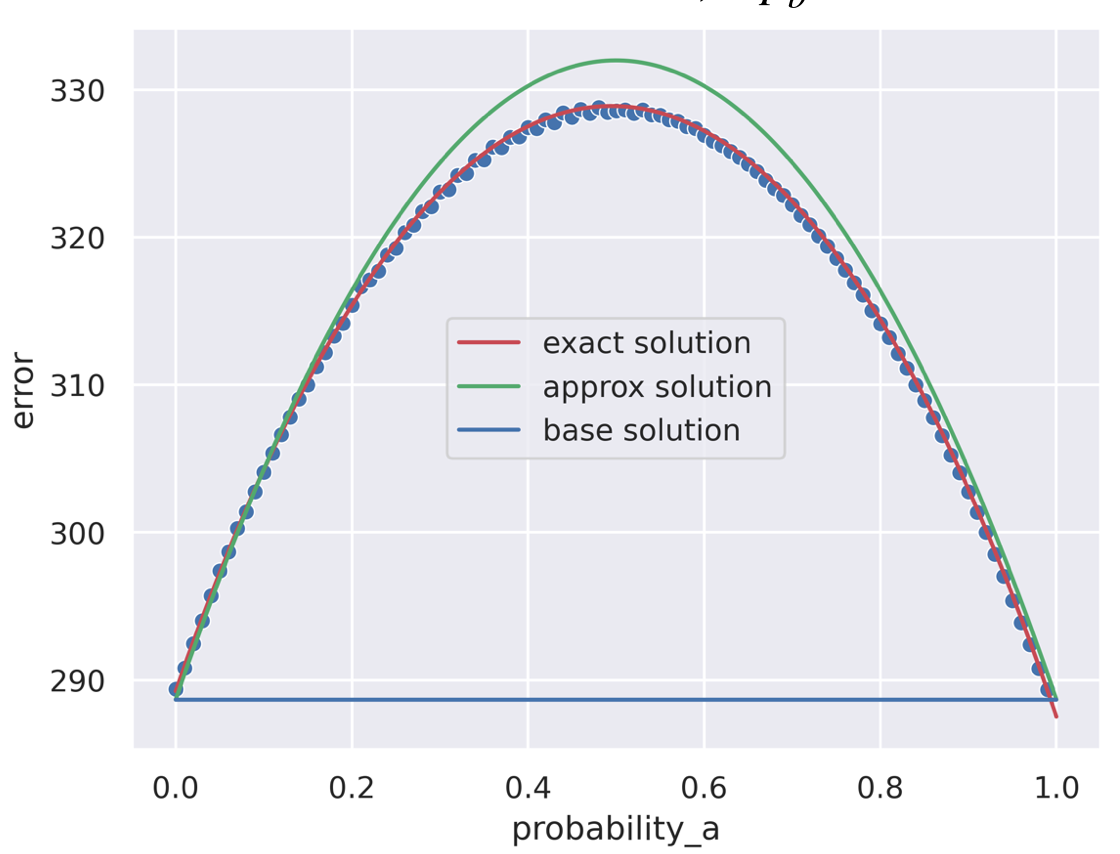
\includegraphics[width = \textwidth]{ neulandMeeting/mapcal_error_validation.png}
			\end{figure}
			\vspace*{-2em}
			{
				\small
				\begin{flalign*}
					p_b & : 0.01    & \\
					N   & : 100'000 & \\
				\end{flalign*}
			}
		\end{column}
	\end{columns}
\end{frame}

\begin{frame}[t]{NeuLAND time and position calibration}
    \vspace*{-2em}
	\begin{columns}[t]
		\begin{column}{0.45\textwidth}
			\begin{block}{\small Time relation:}
				\centering
				$ t = \frac{t_r + t_l}{2} - \frac{L}{2 \cdot \alert{C_e}} + \alert{t_\text{sync}}$
			\end{block}

			\begin{block}{\small Position relation:}
				\centering
				$ x = \frac{\alert{C_e}}{2}\left( t_r - t_l  + \alert{t_\text{offset}} \right)$
			\end{block}
			\flushleft\textbf{Calibration parameters:}
			\begin{itemize}
				\item \alert{$C_e$}  : effective speed of light
				\item \alert{$t_\text{sync}$} : time synchronization among scintillators
				\item \alert{$t_\text{offset}$} : time offset between adjacent PMTs
			\end{itemize}

		\end{column}
		\begin{column}{0.45\textwidth}
			\flushleft\textbf{Calibration using muon tracks:}
			\begin{block}{\small Time and position relation for muon tracks:}
				\centering
				\vspace*{-1.5em}
				\begin{align}
					\small
					x_\mu & = \textcolor{blue}{a^i_x} \cdot z_\mu  + \textcolor{blue}{b^i_x} \\
					y_\mu & = \textcolor{blue}{a^i_y} \cdot z_\mu  + \textcolor{blue}{b^i_y} \\
					t_\mu & = \textcolor{blue}{a^i_t} \cdot z_\mu  + \textcolor{blue}{b^i_t}
				\end{align}
			\end{block}
			\flushleft\textit{\small Calibration parameters for the $i$th muon track in $n$th bar:}
			$$\alert{C^n_e}, \alert{t^n_\text{sync}}, \alert{t^n_\text{offset}},\textcolor{blue}{a^i_x}, \textcolor{blue}{a^i_y}, \textcolor{blue}{a^i_t}, \textcolor{blue}{b^i_x}, \textcolor{blue}{b^i_y}, \textcolor{blue}{b^i_t} $$
			\flushleft\textit{\small Total number of calibration parameters for $m$ muon tracks:} $ 3900 + 6m$
		\end{column}
	\end{columns}
\end{frame}

\begin{frame}[t]{Principle of Millepede algorithm}
    \begin{center}
        \textbf{Linear regression}
    \end{center}
    
\end{frame}

\end{document}
